% Prof. Dr. Ausberto S. Castro Vera
% UENF - CCT - LCMAT - Curso de Ci\^{e}ncia da Computa\c{c}\~{a}o
% Campos, RJ,  2023
% Disciplina: Paradigmas de Linguagens de Programa\c{c}\~{a}o
% Aluno: Gabriel Costa Fassarella


\chapterimage{ScalaH} % Chapter heading image ==>  Trocar este arquivo por outro 1200x468
\chapter{ Programa\c{c}\~{a}o em Scala}
Neste capítulo avançaremos mais ainda na programação em Scala, abordando temas relacionados as classes, funções, listas, vetores e entre outras estruturas apresentadas na linguagem, seguindo os autores \cite{Odersky}, \cite{Sfregola2021} e \cite{Wampler2021}.

   %%%%%%%%======================
    \section{Funções}
    %%%%%%%%======================
    Em programação, uma função é um bloco de código responsável por executar uma instrução específica, recebendo um ou mais valores (parâmetros) como entrada podendo retornar ou não um valor específico.
    
    Funções costumam ser usadas para reduzirem o tamanho do código ou torna-lo mais organizado, gerenciáveis e reutilizáveis. Criando essas funções, é possível encapsular um trecho específico do código, permitindo o programador realizar chamadas da função em outras partes do programa. Isso garante que o código seja mais fácil de ler, de testar e também de manter.
    
    Em Scala, funções são estruturas de primeira classe, ou seja, podem ser atribuídas a variáveis, passadas para outras funções como um argumento e pode ainda ser retornada como valor de outra função.
    
    Na figura abaixo retirada o livro "programming in scala" de \cite{Odersky} é possível identificar a estrutura de uma função em Scala. Segundo \cite{Odersky} as funções são sempre iniciadas usando a palavra-chave "def", seguido pelo seu nome e por um parênteses com seus parâmetros e tipagem. Após isso é necessário especificar o tipo de dado retornado pela função, em seguida basta escrever o corpo que vai apresentar o código dessa função.
    
    \begin{figure}[H]
    	\centering
    	\caption{Estrutura Função}
    	\label{Estrutura Função}
    	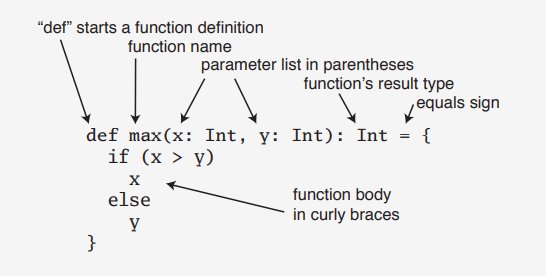
\includegraphics[width=11cm]{func.png} \\
    	Fonte: \cite{Odersky}
    \end{figure}

	No exemplo acima existe uma função chamada max que retorna um valor int, ainda possui dois parâmetros: x e y, ambos com tipagem int. Nessa função, o retorno será decidido por alguma operação dentro das chaves, nesse caso um if, que escolhe entre x e y.
	
	Uma vez criada a função basta chama-la no código principal, para isso é necessário escrever o seu nome e os parâmetros desejados: 
	
	Neste caso:
	\begin{lstlisting}
		max(5, 7)
		
		[Running] 7
	\end{lstlisting}

	Vale lembrar que todo o código Scala é rodado dentro de uma função denominada main, o mesmo ocorre em outras linguagens como C por exemplo. A estrutura do main é dada da seguinte forma:
	
	\begin{lstlisting}[breaklines]
		object hello {
			def main(args: Array[String]): Unit = {
				println("Hello, world!")	
		}	
	}
	\end{lstlisting}
	
	Para realizar um hello world em Scala é necessário primeiro declarar uma classe, para isso se utiliza a expressão "object [nome da classe]", dessa forma podemos criar a função denominada main, onde será rodado o código em Scala. Usaremos como parâmetro o args que é um array de strings, dessa forma será passado uma série de argumentos de linhas de comandos para o código. Além disso é utlizado o tipo de dado Unit como saída, indicando uma saída vázia. Após isso basta utilizar o println como já visto antes.

		\section{Classes}
	
	Segundo \cite{Sfregola2021} classes são estruturas fundamentais para linguagens orientadas a objetos, uma vez que elas são utilizadas para definir um objeto. Elas são extremamente usadas para encapsular dados e alguns comportamentos relacionados entre si.
	
	Para definir uma classe basta usar a palavra-chave 'class' seguida de seu nome.
	Exemplo:
	
	\begin{lstlisting}[breaklines]
	class individuo(nome: String, idade: Int) {
		def saudacao(): Unit = {
			println(s"Ola, meu nome e $nome e eu tenho $idade anos.")
		}
			
		def despedida(nome2: String): Unit = {
			println(s"Adeus $nome2, foi um prazer te conhecer!")
		}
	}
		
	def main(args: Array[String]) = {
		val julio = new individuo("Julio" , 15)
			
		julio.saudacao()
		julio.despedida("Gabriel")
	}
		
	[Running]
	Ola, meu nome e Julio e eu tenho 15 anos.
	Adeus Gabriel, foi um prazer te conhecer!
	\end{lstlisting}

	Note que no exemplo dado inicialmente foi criada a classe "individuo" junto de suas entradas, nesse caso o nome e a idade do individuo. Após isso, foram criadas algumas funções, nesse caso chamadas de métodos, sendo esses o método saudacao, que ira realizar um print com o nome e idade, e o outro método sendo o despedida, que irá receber uma entrada, sendo essa um novo nome que será printada no código. Já no main é realizado a declaração da classe e suas respectivas chamadas.

   %%%%%%%%======================
    \section{Listas}
    %%%%%%%%======================

	Segundo \cite{Sfregola2021} em Scala, listas são uma reunião de elementos/dados que são imutáveis de um mesmo tipo. Ou seja, uma vez criada uma lista, não é possível altera-la, porém todos os métodos possíveis de adicionar ou remover elementos de uma lista retornam uma nova lista com as alterações efetuadas.
	
	Para criar uma lista, é necessário utilizar a classe list ou uma sintaxe construtora de listas.
	
	Exemplo de uma lista com 3 elementos:
	
	\begin{lstlisting}
	def main(args: Array[String]) = {
		val lista1 = List(1, 2, 3)
	
		val lista2 = 4 :: 5 :: 6 :: Nil
	
		val lista3 : List [Int] = List (7, 8, 9)
	
		println(lista1)
	
		println(lista2)
	
		println(lista3)
	}

	[Running] 
	List(1, 2, 3)
	List(4, 5, 6)
	List(7, 8, 9)
	\end{lstlisting}
	
	Note que na primeira linha foi necessário utilizar a classe "List" com o objetivo de criar a lista com os 3 números inteiros solicitados. Já na segunda foi utilizada uma sintaxe construtora de lista, sendo que nela o operador "::" adiciona elementos a lista e o operador "Nil" é usado para representar uma lista vazia. E por último na terceira linha também é usada a classe "List", porém nesse caso é identificado o tipo dos valores da lista.
	
	Ainda é possível mostrar como saída os valores da lista por índice, para isso basta identificar a posição que deseja mostrar para o usuário. Vale lembrar que a contagem dos índices sempre começa pelo valor 0.
	
	Exemplo:
	\begin{lstlisting}
		def main(args: Array[String]) = {
			val lista1 = List(1, 2, 3)
			
			println(lista1(0))
			println(lista1(1))
			println(lista1(2))
		}
	
		[Running] 
		1
		2
		3
	\end{lstlisting}

	\subsection{Operações}
	
	Em Scala é muito comum o uso das operações com listas, visto a sua alta capacidade de utilização, permitindo o programador efetuar uma série de manipulações diferentes de maneira simples e extremamente eficiente.
	
	Considerando as listas: lista1 = (1,2,3) e a lista2 = (4, 5, 6), veja alguns exemplos de operações com essas listas:
	
	\begin{lstlisting}[breaklines]
		// concatenacao
		val lista3 = lista1 ++ lista2
		[Running] List(1, 2, 3, 4, 5, 6)
		
		// adicionando elementos
		val lista4 = lista1 :+ 4 
		[Running] List(1, 2, 3, 4)
		
		// removendo elementos
  		val lista5 = lista1.filterNot(_ == 3) //remove o elemnto 3
  		[Running] List(1, 2)
  		
  		// mapeamento
  		val lista6 = lista1.map(_ * 2) //multiplica a lista por 2
  		[Running] List(2, 4, 6)
  		
  		// reduzindo elementos
  		val red = lista2.reduce(_ + _) //soma todos os elementos
  		[Running] 15
	\end{lstlisting}

    %%%%%%%%======================
    \section{Tuplas}
    %%%%%%%%======================

	Segundo \cite{Odersky}: "Assim como as listas, as tuplas são imutáveis, mas ao contrário das listas, as tuplas podem conter diferentes tipos de elementos". Ou seja, não é possível alteras os valores de uma tupla, porém diferente das listas, uma mesma tupla pode conter um dado do tipo inteiro e outro dado do tipo string por exemplo.
	
	Para criar uma tupla em Scala é necessário inicia-la usando parênteses separando os seus elementos por vírgula.
	
	Exemplo de uma tupla composta por uma string e um float:
	
	\begin{lstlisting}
		def main(args: Array[String]) = {
			val tupla1 = ("Ola!", 3.14)
			
			println(tupla1)
		}
	
		[Running] (Ola!,3.14)
	\end{lstlisting}

	Os elementos do interior de uma tupla podem ser acessados por meio da notação "NomeDaTupla.\_Posição", sendo que a posição diferente de uma lista começa pelo número 1.
	
	\begin{lstlisting}
		def main(args: Array[String]) = {
			val tupla1 = ("Ola!", 3.14)
			
			println(tupla1._1)
			println(tupla1._2)
		}
	
		[Running]
		Ola!
		3.14
	\end{lstlisting}

	\subsection{Operações}
	Assim como as listas, as tuplas apresentam algumas operações possíveis que podem ser extremamente uteis durante a programação. Considerando a tupla val tupla1 = ("Ola!", 3.14), veja alguns exemplos das operações mais comuns envolvendo tuplas em Scala.
	
	\begin{lstlisting}[breaklines]
		//Desestruturar tupla
		val (msg, pi) = minhaTupla //atribui o valor da tupla a variaveis individuais
		
		println(msg)
		println(pi)
		
		[Running] 
		Ola!
		3.14
		
		//Concatenar tuplas
		val tupla2 = ("x", 2)
		val tupla3 = tupla1 ++ tupla2
		println(tupla3)
		
		[Running] (Ola!,3.14,x,2)
		
		//Verificar Tamanho
		val range = tupla1.size
		println(range)
		
		[Running] 2
		
		//Transformar tupla em lista
		val tupla1 = ("Ola!", "mundo")
		val lista = tupla1.toList
		println(lista)
		
		[Running] List(Ola!, mundo)
	\end{lstlisting}


   %%%%%%%%======================
    \section{Set}
    %%%%%%%%======================

	De acordo com \cite{Odersky}, em Scala um set é uma estrutura responsável por agrupar um conjunto de elementos porém sem permitir uma "duplicata" dos mesmos, ou seja, cada elementos presente em um set é único e não possui uma cópia de si mesmo. O conteúdo de um set é armazenado em uma ordem não definida e não possui nenhum índice associado a ele.
	
	Para se implementar um set é necessário usar uma estrutura de dados chamada de "hash table". Isso permite que muitas operações como as de adição, remoção e verificação possam ser executadas constantemente, fazendo com que os sets sejam extremamente eficazes na manipulação de big data.
	
	Exemplo:
	
	\begin{lstlisting} [breaklines]
		val materias = Set("fisica", "calculo", "programacao")
		
		println(materias)
		
		[Running] Set(fisica, calculo, programacao)
	\end{lstlisting}

	Em Scala, a estrutura set apresenta 2 tipos, o tipo mutável e o tipo imutável. O primeiro como o próprio nome diz não podem ser mudados depois de criados, ou seja, qualquer operação de adição ou remoção de elementos, por exemplo, feita em um set imutável retorna um novo set para o usuário. Já o set mutável é o oposto, ou seja, são estruturas que podem ser modificadas depois de sua criação, porém para cria-las é necessário utilizar a biblioteca "scala.collection.mutable.Set".
	
	Operações com set imutável: 
	
	\begin{lstlisting}[breaklines]
		//criando set
		val seq = Set(1, 2, 3)
		
		//adicionando elemento 
		val newseq = seq + 4
		
		//removendo elemento
		val remseq = seq - 3
		
		//unindo set
		val newset = Set(4, 5, 6)
		val uniset = seq ++ newset
		
		//verifica a existencia de um elemento
		val existe1 = seq.contains(1)
		
		//verfica o tamanho do set
		val range = seq.size
	\end{lstlisting}

	Operações com set mutável: 
	
	\begin{lstlisting}
		//importando biblioteca
		import scala.collection.mutable.Set
		
		//criando set vazio
		val seq = Set[Int]()
		
		//adicionando elemento
		seq += 7
		seq += 8
		seq += 9
		
		//removendo elemento
		seq -= 9
		
		//atualizando elemento
		seq.update(7, 3) //substitui o 7 pelo 3
		
		//verificando a existencia de um elemento
		seq.contains(8)
		
		//limpando set
		seq.clear()
	\end{lstlisting}

   %%%%%%%%======================
    \section{Map}
    
    Em Scala, "map" é uma coleção de elementos que armazena chaves e valores relacionados. É um conjunto de dados extremamente eficiente para realizar consultas, pesquisas e operações se baseando nas chaves.
    
    Como criar um map em Scala:
    
    \begin{lstlisting}
    	val map = Map("key1" -> 1, "key2" -> 2, "key3" -> 3)
    	
    	println(map("key1"))
    	
    	[Running] 1
    	
    	
    \end{lstlisting}

	Para criar uma estrutura map em Scala, basta utilizar a classe "Map", e indicar as chaves e longo em seguida o valor específico dessa chave.
	
	Algumas operações com map:
	\begin{lstlisting}[breaklines]
		val map = Map("key1" -> 1, "key2" -> 2, "key3" -> 3)
		
		//update: rertorna um novo map com valores atualizados
		map + (key4 -> 4)
		
		//remove: retorna um novo map sem o par da chave
		map - "key1"
		
		//contains: verifica se o map possui uma chave
		map.contains(key2)
		
		//isEmpty: verifica se o map esta vazio
		map.isEmpty
		
		//size: retorna o tamanho do map
		map.size
		
		//keySet: retorna todas as chaves do map
		map.keySet
		
		//values: retorna todos os valores do map
		map.values
	\end{lstlisting}
    %%%%%%%%======================

	\section{Array}
	
	Segundo \cite{Odersky}, em Scala um array é um conjunto de elementos armazenados e uma sequência fixa, e diferente das outras coleções imutáveis como set e lista, é possível alterar os valores presentes em um array mesmo após a sua criação, ou seja, o array é uma estrutura mutável.
	
	Em Scala, todo array apresenta uma estrutura um tamanho fixo determinada determinado na sua criação, sendo que todos os seus elementos devem apresentar o mesmo tipo de dado, ou seja, array é uma estrutura de tipo homogêneo.
	
	Como criar um array:
	\begin{lstlisting}
		val array1: Array[Int] = Array(1,2,3)
		
		println(array1(2))
		
		[Running] 3
	\end{lstlisting}

	Para criar um array basta utilizar a classe e indicar os seus elementos.
	
	Algumas operações:
	\begin{lstlisting}
		//criando array
		val array1: Array[Int] = Array(1,2,3)
		
		//acessa o valor do indice informado
		array1(0)
		
		//modifica elemento no indice informado
		array1 = 6
		
		//tamanho do array
		array1.length
	\end{lstlisting}

